\documentclass{article}
\usepackage{minted}
\usepackage{xcolor}
\usepackage{graphicx}
\graphicspath{{./images/}}
\definecolor{LightGray}{gray}{0.9}
\title{Software Development Week 4}
\author{Nathan Le Brun}
\date{\today}

\begin{document}
    \maketitle
    VSV Id: 107027
    
    \section[Task 1]{Task 1 - For Loops}
        \subsection{For Loop}
            \begin{minted}[breaklines, bgcolor=LightGray]{php}
<?php
  for ($i = 1; $i >= 10; $i++) {
    echo "$i <br>"
  }
?>
            \end{minted}
            \begin{figure}[h]
                \centering
                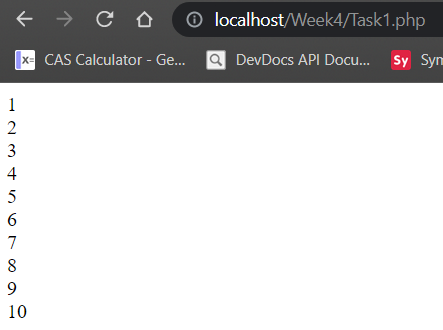
\includegraphics{Task1A}
                \caption{The output of the code shown above}
            \end{figure}
        \subsection{BMI Calculator}
            
            \begin{minted}[breaklines, bgcolor=LightGray]{php}
<?php
  function calc_bmi(float $height, float $weight): float {
    return round($weight / ($height * $height), 1);
  }
  
  function classify_bmi(float $bmi): string {
    if ($bmi < 18.5) {return "Underweight";}
    if ($bmi > 30) {return "Obese";}
    if ($bmi < 24.9) {return "Normal Weight";}
    return "Overweight";
  }

  function return_bmi_result(string $name, float $height, float $weight): string {
    $bmi = calc_bmi($height, $weight);
    return "$person weighs $weight and is $height metres tall. $person's BMI is $bmi, which classifies them as " . classify_bmi_result($bmi);
  }
  $people = [["Foo", 1.692, 65.7], ["Bar", 1.784, 72.9], ["Baz", 1.72, 47]];
  for ($i = 0; $i < 3; $i++) {
    $person = $people[$i];
    $name = $person[0];
    $height = $person[1];
    $weight = $person[2];
    echo return_bmi_result($name, $height, $weight) . "<br>";
  }
?>
            \end{minted}
            \begin{figure}[h]
                \centering
                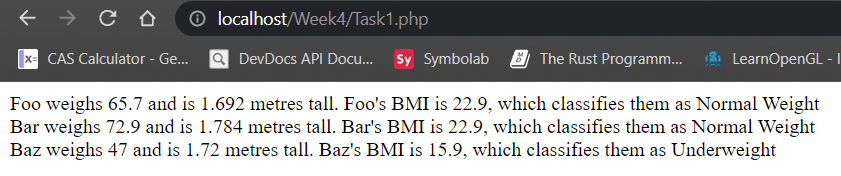
\includegraphics[width=1.0\textwidth]{Task1B}
                \caption{The output of the code shown above}
            \end{figure}
    \section[Task 2]{Task 2 - Arrays}
        \subsection{Difference between an associative and indexed array}
            The difference between an associative and indexed array is that an indexed array has numerical keys whereas an associative array can have keys of any type and is closer to a collection of key-value pairs
        \subsection{Different Arrays}
            \begin{enumerate}
                \item Array types:
                \begin{enumerate}
                    \item Array B is an indexed array
                    \item Array A is an associative array
                \end{enumerate}
                \item The keys for Array A are \verb|Red|, \verb|White|, \verb|Green| and \verb|Blue|
                \item The values of Array B are \verb|22.7|, \verb|28.5| and \verb|22.1|
            \end{enumerate}
        \subsection{Two Arrays For Loop}
            \begin{minted}[breaklines, bgcolor=LightGray]{php}
<?php
  $arrayA = array();
  $arrayB = array();
  
  $arrayA["Red"] = "#FF0000";
  $arrayA["White"] = "#FFFFFF";
  $arrayA["Green"] = "#008000";
  $arrayA["Blue"] = "#0000FF";
  
  $arrayB[0] = 22.7;
  $arrayB[1] = 28.5;
  $arrayB[2] = 22.1;
  
  echo "arrayA" . "<br>";
  foreach($arrayA as $color) {
    echo $color . "<br>";
  }
  
  echo "arrayB" . "<br>";
  for($i = 0; $i < count($arrayB); $i++) {
    echo $arrayB[$i] . "<br>";
  }
?>
            \end{minted}
            \begin{figure}[h]
                \centering
                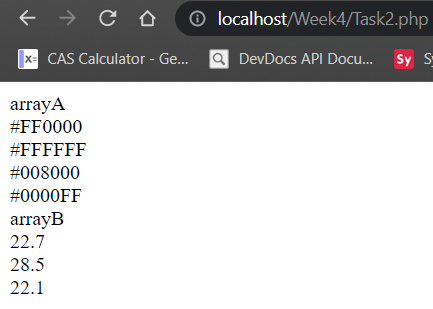
\includegraphics[width=1.0\textwidth]{Task2C}
                \caption{The output of the code shown above}
            \end{figure}
        
\end{document}